\documentclass[12pt]{article}

\usepackage{amsmath}

\usepackage{graphicx}

\usepackage{hyperref}

\usepackage{graphicx}
\graphicspath{ {./Pics/} }

\usepackage{listings}
\usepackage{color}

\definecolor{dkgreen}{rgb}{0,0.6,0}
\definecolor{gray}{rgb}{0.5,0.5,0.5}
\definecolor{mauve}{rgb}{0.58,0,0.82}

\lstset{frame=tb,
  language=C,
  aboveskip=3mm,
  belowskip=3mm,
  showstringspaces=false,
  columns=flexible,
  basicstyle={\small\ttfamily},
  numbers=none,
  numberstyle=\tiny\color{gray},
  keywordstyle=\color{blue},
  commentstyle=\color{dkgreen},
  stringstyle=\color{mauve},
  breaklines=true,
  breakatwhitespace=true,
  tabsize=3
}

\usepackage[utf8]{inputenc}

\title{Computer Architecture}
\author{Yuqiao Meng}
\date{2022-1-28}

\begin{document}

\maketitle

\newpage
\tableofcontents

\newpage

\section{Overview}
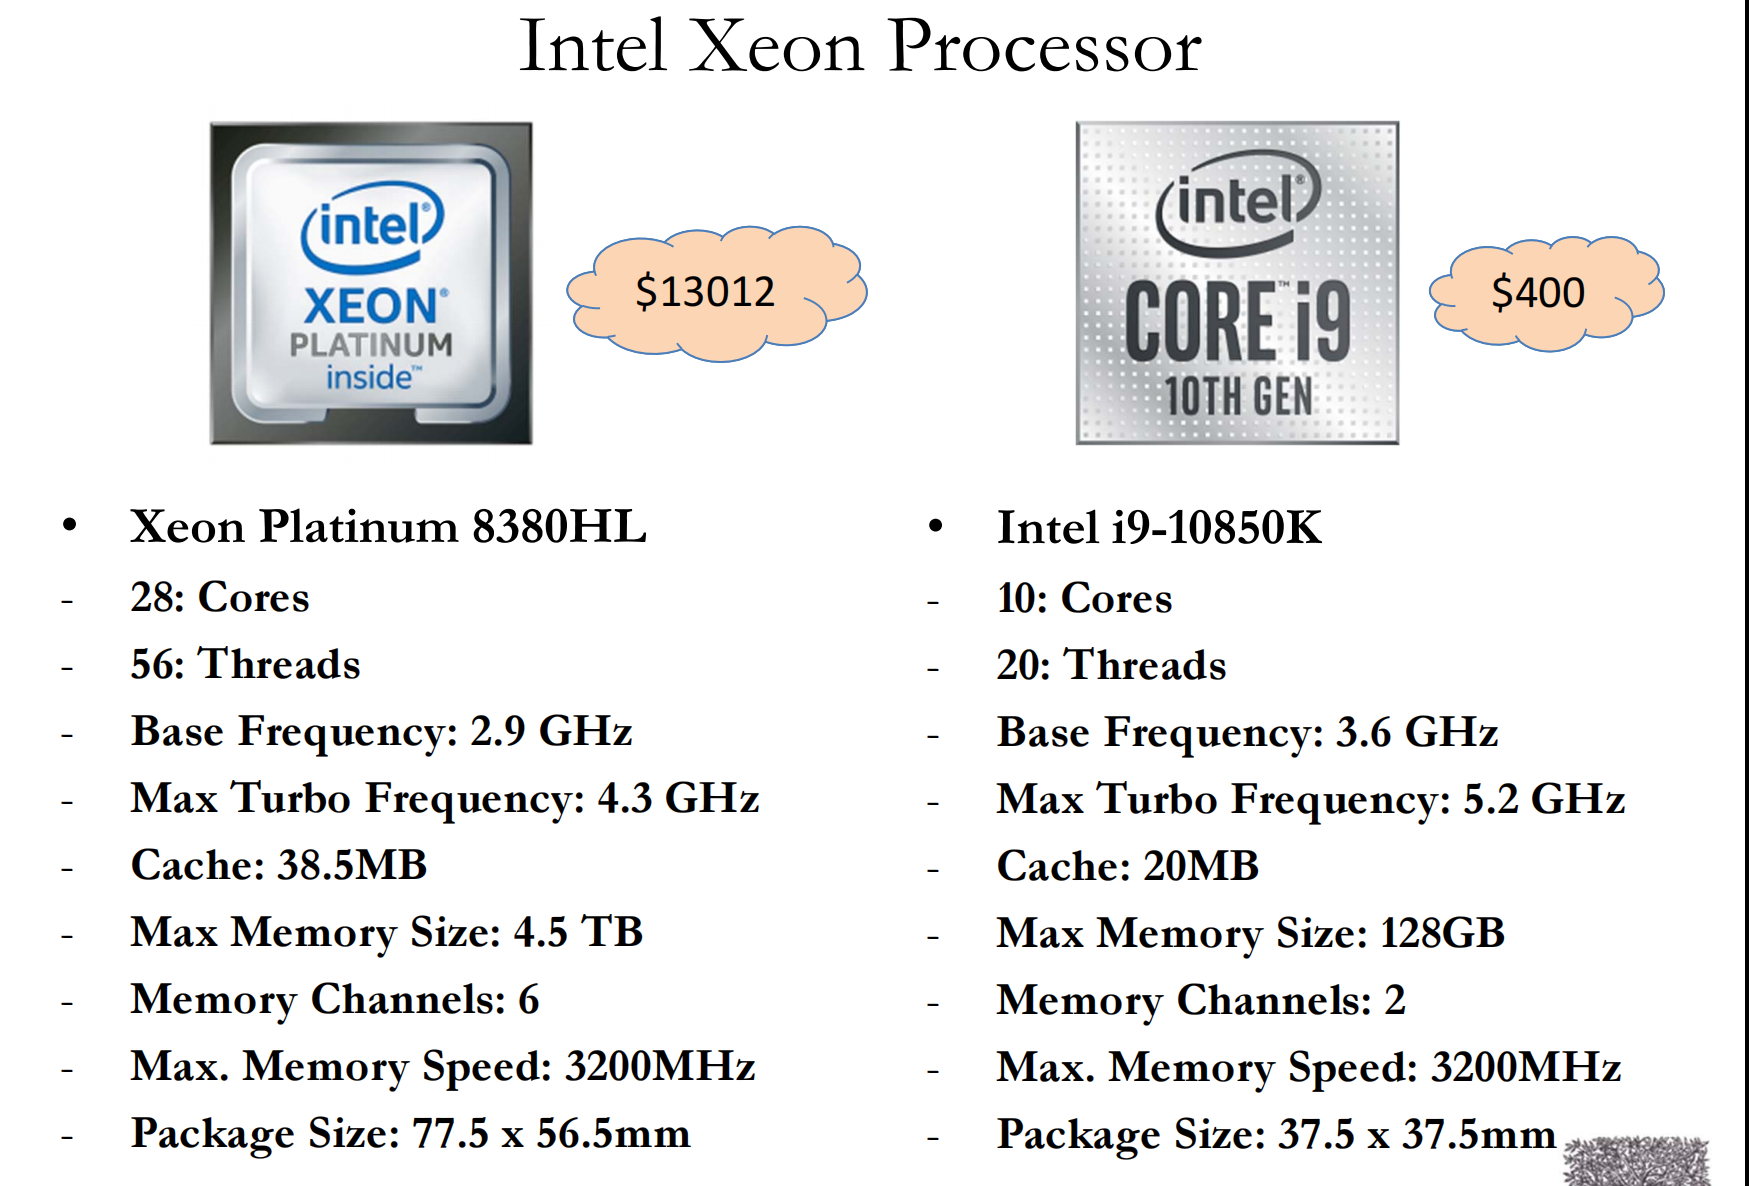
\includegraphics[width=\textwidth]{ProcessorOverview.png}
\subsection{Why the prices of two processors differs?}
\begin{enumerate}
    \item The prices increase exponentially as the number of Cores and Threads increase. That's because every core has a bad possibility, so the difficult of making a processor with many cores much harder.
    \item Significant: The memory Chaneels of XEON is three times by i9, which means it has three times as many pins as i9 has.
\end{enumerate}

\section{Digital Design}
\subsection{Abstraction}
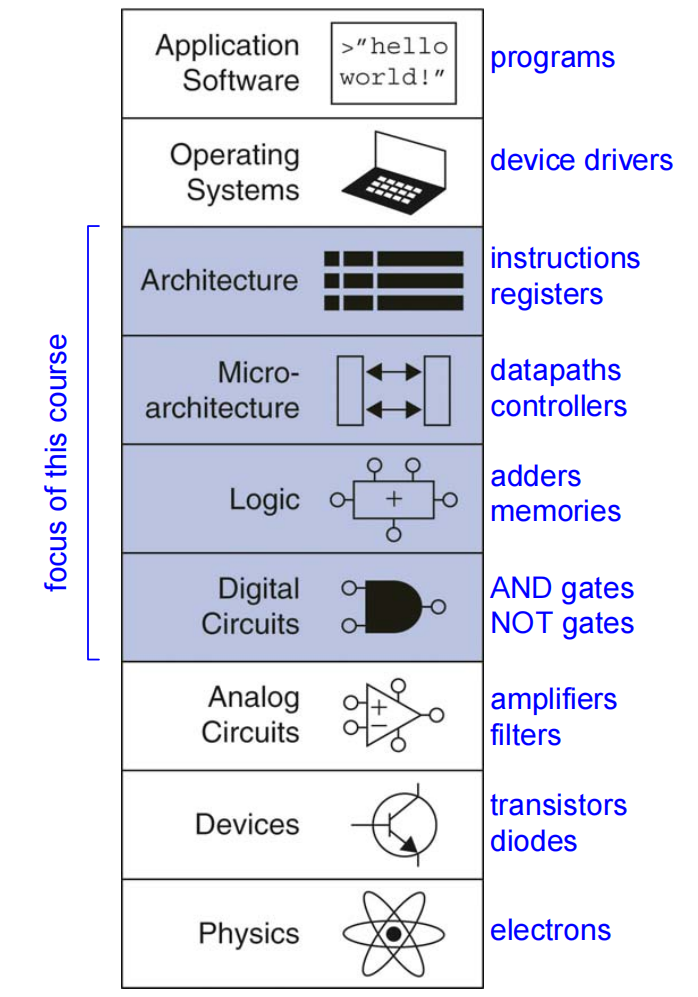
\includegraphics[width=0.6\textwidth]{Abstraction.png}
\subsection{The Digital Abstraction}
\begin{itemize}
    \item Most physical variables are continuous \begin{itemize}
        \item Voltage on a wire
        \item Frequency of an oscillation
        \item Position of a mass
    \end{itemize}
    \item Digital abstraction considers discrete subset of values
\end{itemize}
\subsection{Digital Discipline: Binary Values}
\begin{itemize}
    \item Two discrete Values: \begin{itemize}
        \item 1's and 0's
        \item 1, true, high
        \item 0, false, low
    \end{itemize}
    \item 1 and 0: voltage levels, rotating gears, fluid levels
    \item Digital circuits use voltage levels to represent 1 and 0
\end{itemize}
\subsection{Decimal to Binary Conversion}
Method: repeatedly divided by 2, remainders goes in next most significant bit
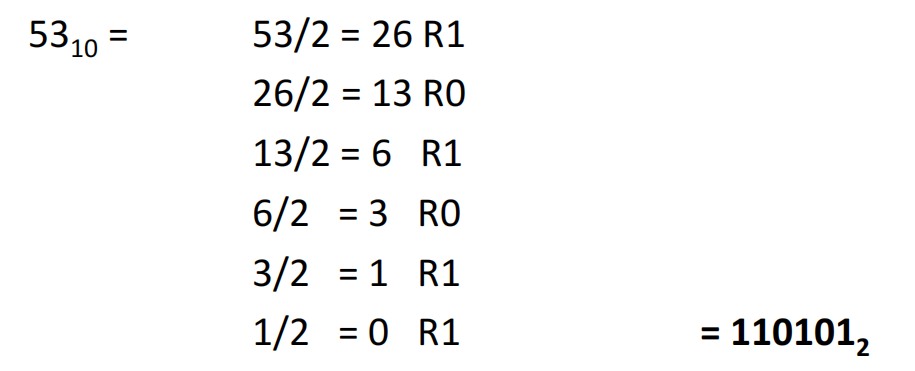
\includegraphics[width=\textwidth]{DecimalToBinary.png}
\subsection{Signed Binary Numbers}
\subsubsection{Sign/Magnitude Numbers}
Problems
\begin{itemize}
    \item Has two 0 values, positive 0 and negative 0
    \item Addition of a negative and a postive will fail
\end{itemize}
\subsubsection{Two's Complement Numbers}
Conversion from positive to negative:
\begin{itemize}
    \item Invert every bit
    \item Add 1
\end{itemize}
\subsection{Logic Gates}
\begin{itemize}
    \item AND 
    \item OR 
    \item XOR
    \item NAND
    \item NOR
    \item XNOR
\end{itemize}
\subsection{Logic levels}
Discrete voltages represent 1 and 0, but there is noise that will degrade the signal
\subsubsection{Noise Margins}
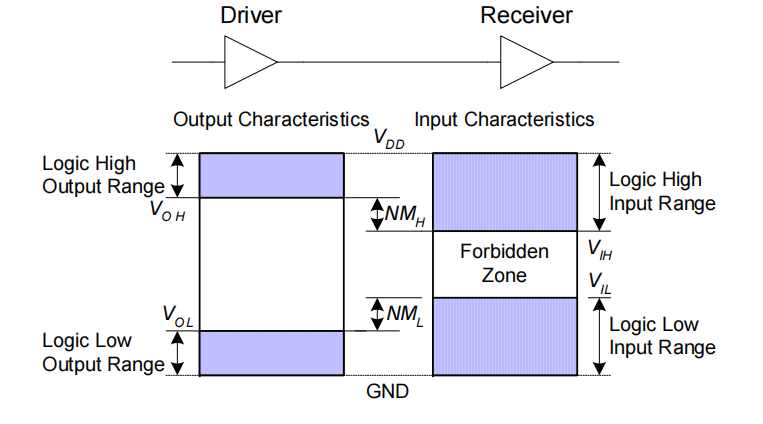
\includegraphics[width=\textwidth]{NoiseMargins.png}
\begin{itemize}
    \item High Noise Margin: $NM_H = V_{OH}-V_{IH}$
    \item Low Noise Margin: $NM_L = V_{OL}-V_{IL}$
\end{itemize}
\subsubsection{Transfer Characteristics}
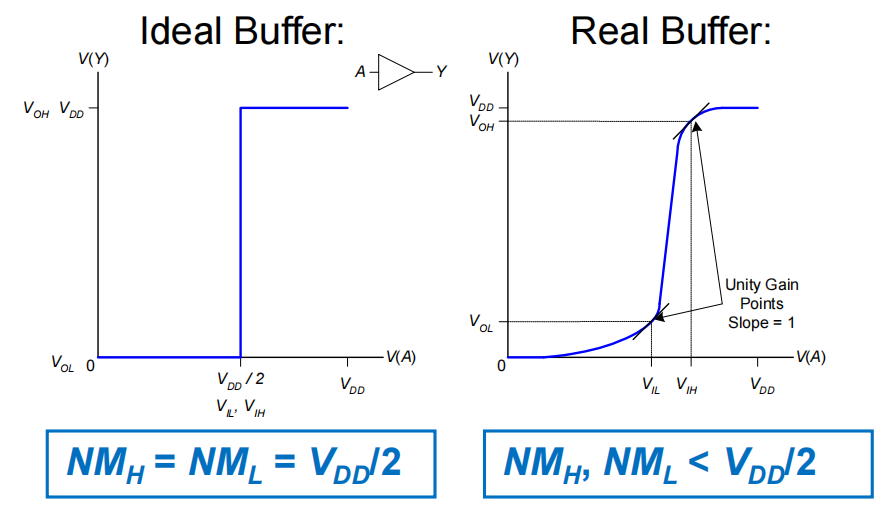
\includegraphics[width=\textwidth]{TransferCharacteristics.png}
\subsection{MOS Transistor}
\begin{itemize}
    \item Polysilicon Gate: control the transistor
    \item Oxide insulator: keep electrons to form a path for electricity
    \item Doped Silicon
\end{itemize}
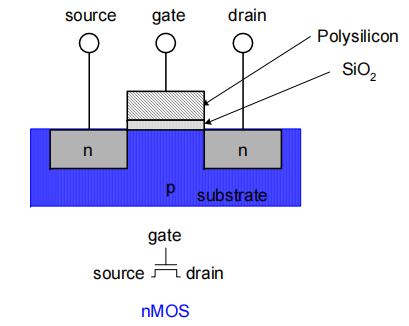
\includegraphics[width=\textwidth]{Transistor.png}
\subsubsection{nMOS}
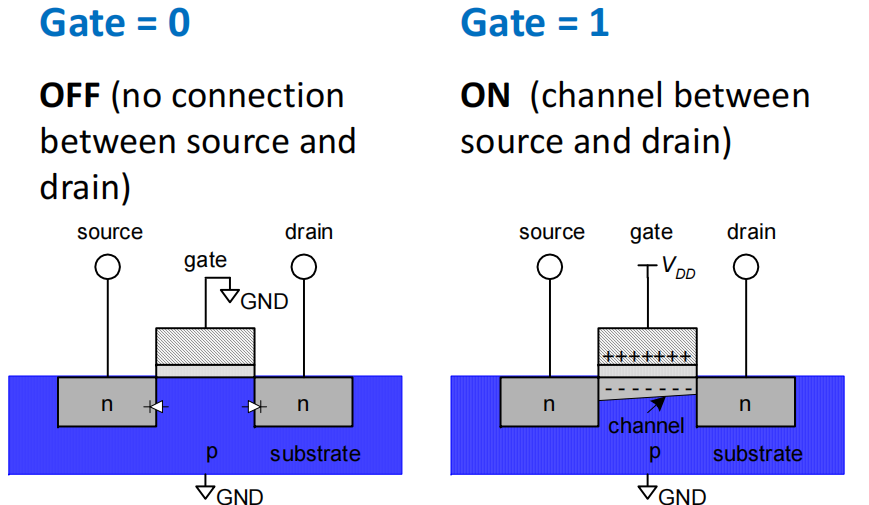
\includegraphics[width=\textwidth]{nMOS.png}
\subsubsection{pMOS}
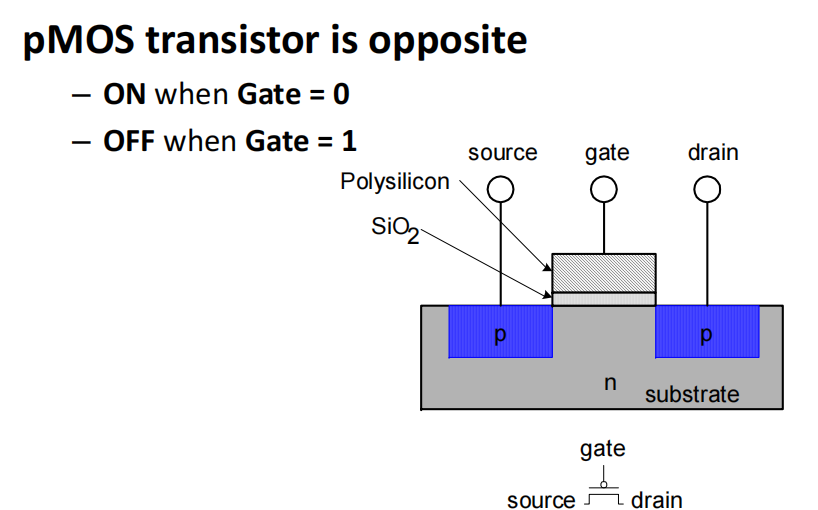
\includegraphics[width=\textwidth]{pMOS.png}
\subsubsection{Why do we need two types of MOS?}
\begin{itemize}
    \item nMOS: pass good 0's, so connect source to GND
    \item pMOS: pass good 1's, so connect source to VDD
\end{itemize}
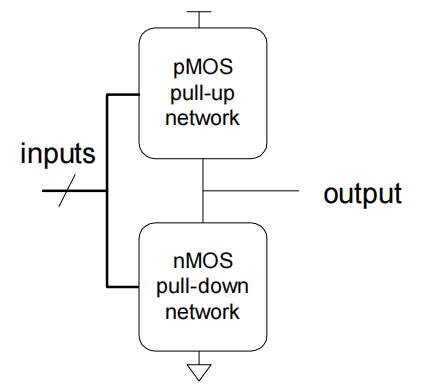
\includegraphics[width=\textwidth]{TransistorFunction.png}
\subsection{cMos NAND Gate}
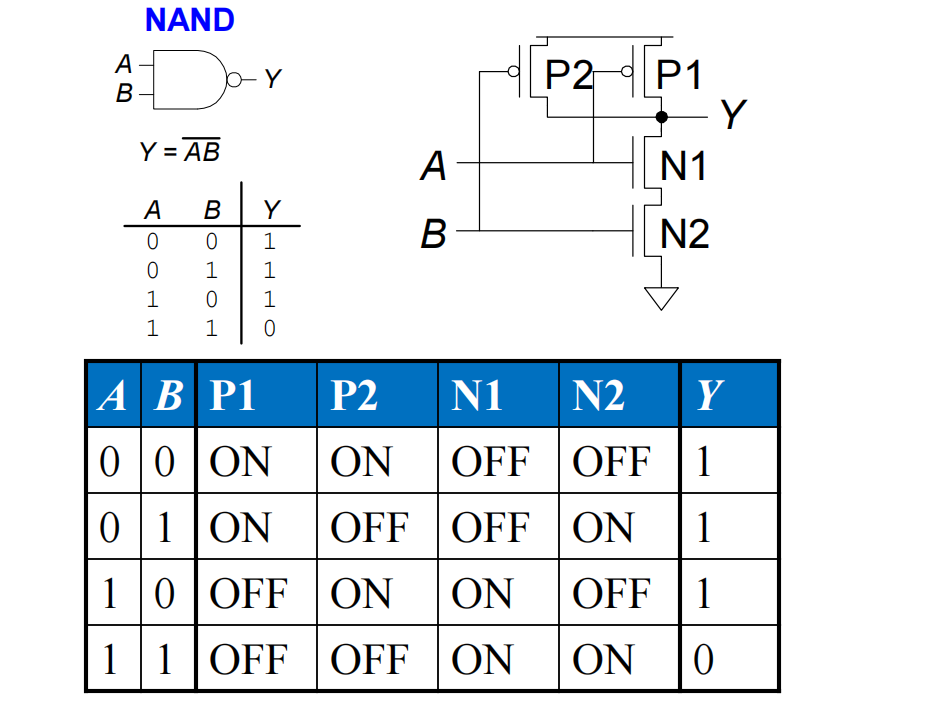
\includegraphics[width=\textwidth]{cMosNANDGate.png}
\subsection{Pseudo-nMOS Gates}
\begin{itemize}
    \item Replace pull-up network with weak pMOS transistor that is always on
    \item Tradeoff: need more energy
\end{itemize}
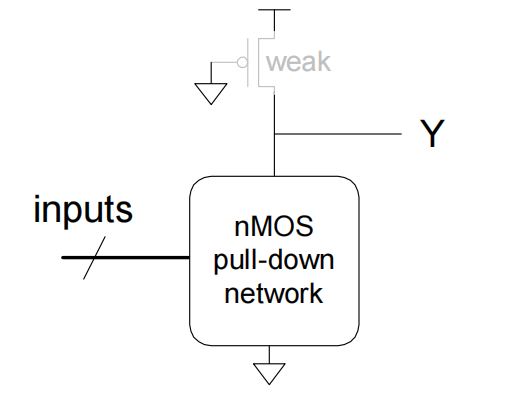
\includegraphics[width=\textwidth]{Pseudo-nMos.png}
\subsection{Power Consumption}
\begin{itemize}
    \item Dynamic power consumption: Power to charge transistor gate capacitances \begin{itemize}
        \item $P_{Dynamic} = \frac{1}{2}CV_{DD}^2f$
        \item f: Frequency
        \item $CV_{DD}^2f$: energy to charge a capacitance
    \end{itemize}
    \item Static power consumption \begin{itemize}
        \item power consumed when no gates are switching
        \item caused by quiescent supply current $I_{DD}$(there is more and more current leackage for transistor is smaller and smaller, and the distance between source and drain is shorter and shorter, so there is more and more quiescents leaked)
        \item $P_{static} = I_{DD}V_{DD}$
    \end{itemize}
    \item $P = \frac{1}{2}CV_{DD}^2f + I_{DD}V_{DD}$
\end{itemize}
\subsection{Circuits}
\subsubsection{Composition}
\begin{itemize}
    \item inputs
    \item outputs
    \item functional specification
    \item timing specification
\end{itemize}
\subsubsection{Types}
\begin{itemize}
    \item Combinational \begin{itemize}
        \item Memoryless
        \item output $\to$ current value of inputs
    \end{itemize}
    \item Sequential \begin{itemize}
        \item has memory
        \item output $\to$ previous and current value of inputs
    \end{itemize}
\end{itemize}
\subsubsection{Definitions}
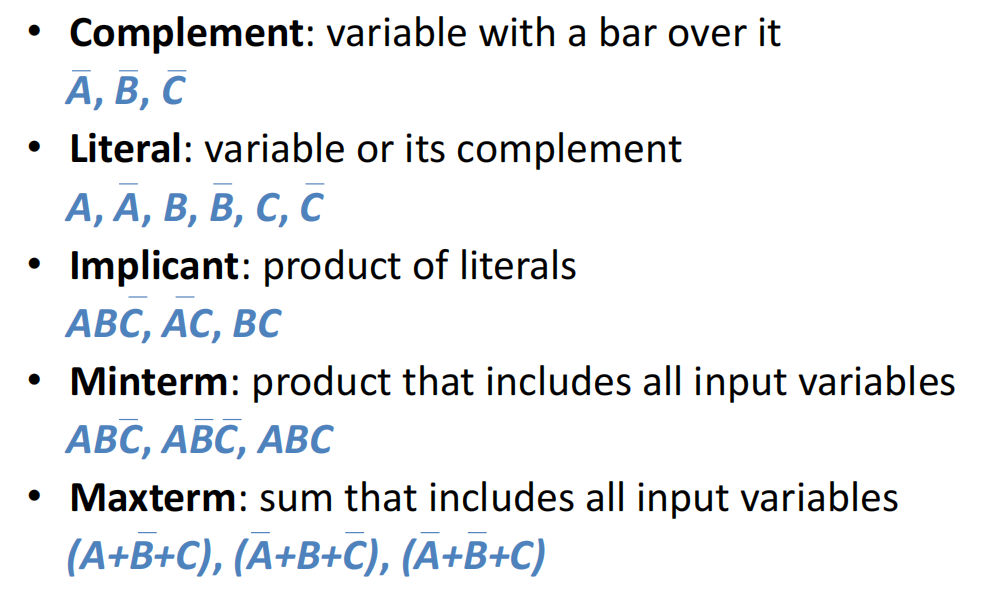
\includegraphics[width=\textwidth]{SomeDefinitions.png}
\subsubsection{SOP Forms}
\begin{itemize}
    \item Each row has a minterm(products of literals)
\end{itemize}
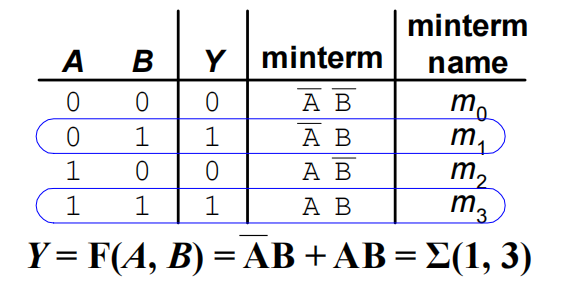
\includegraphics[width=\textwidth]{SOPForm.png}
\subsubsection{POS Forms}
\begin{itemize}
    \item Each row has a maxterm(sum of literals)
\end{itemize}
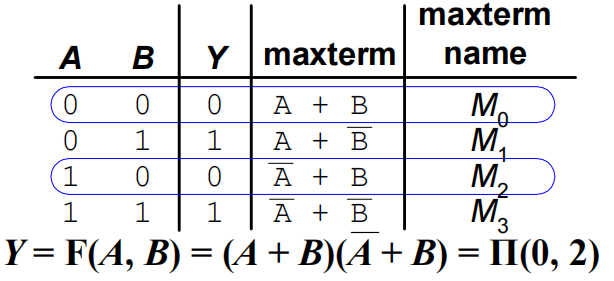
\includegraphics[width=\textwidth]{POSForm.png}
\subsubsection{SOP \& POS Forms}
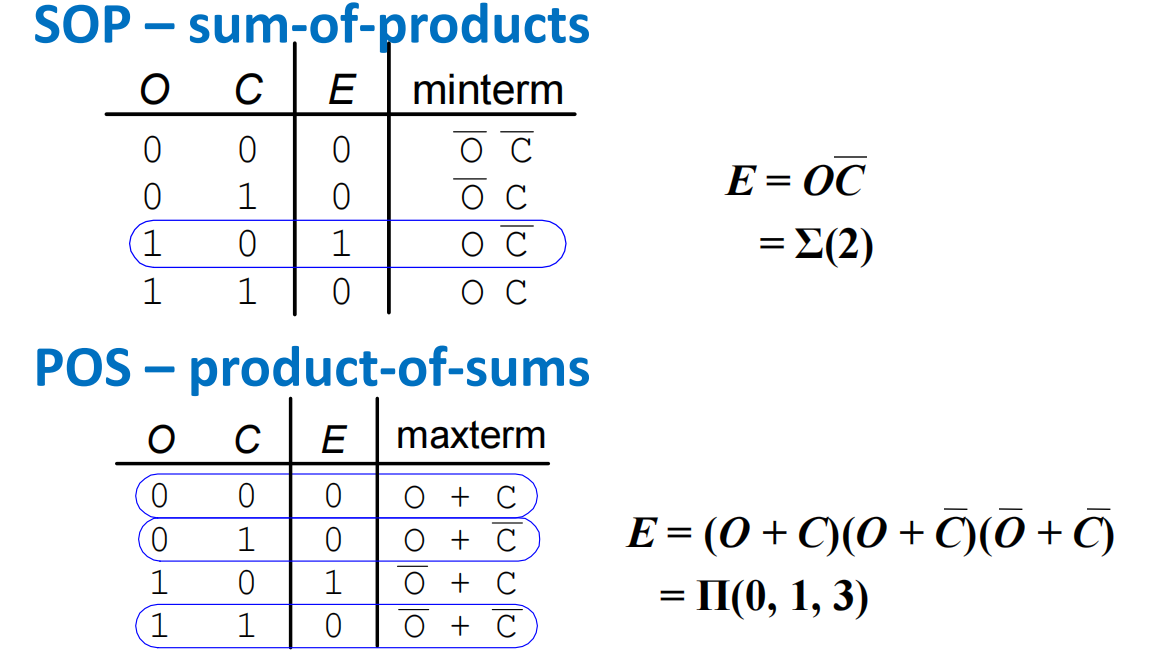
\includegraphics[width=\textwidth]{SOP&POS.png}
\subsection{Boolean}
\subsubsection{Axiom}
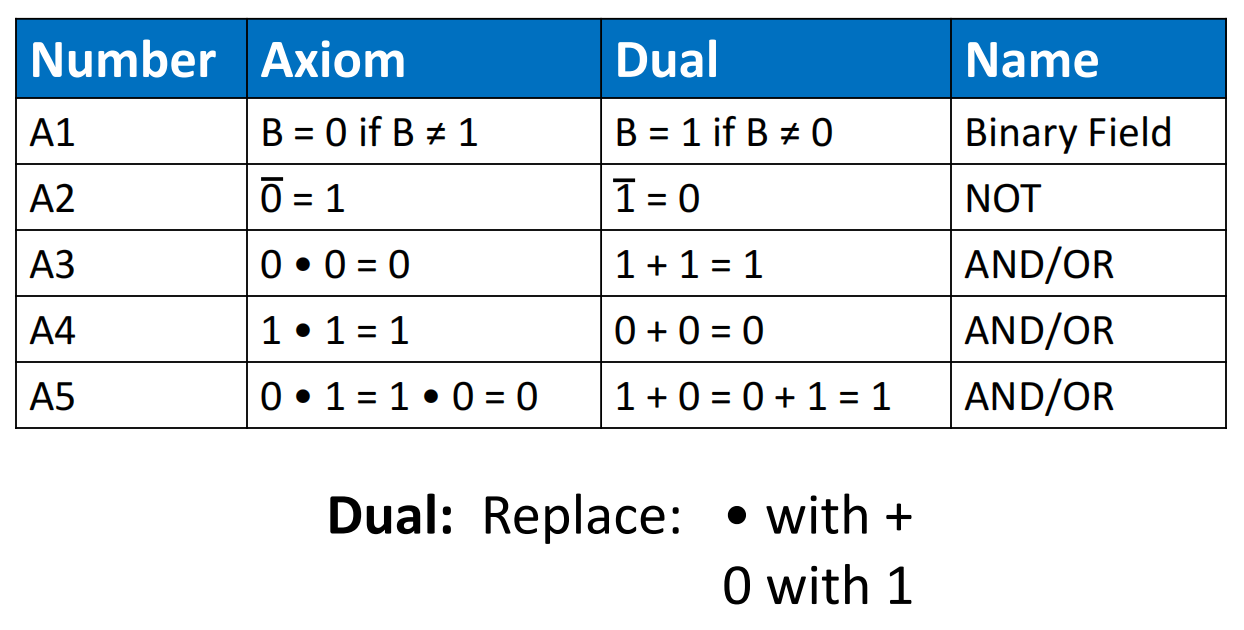
\includegraphics[width=\textwidth]{Axioms.png}
\subsubsection{Theorem}
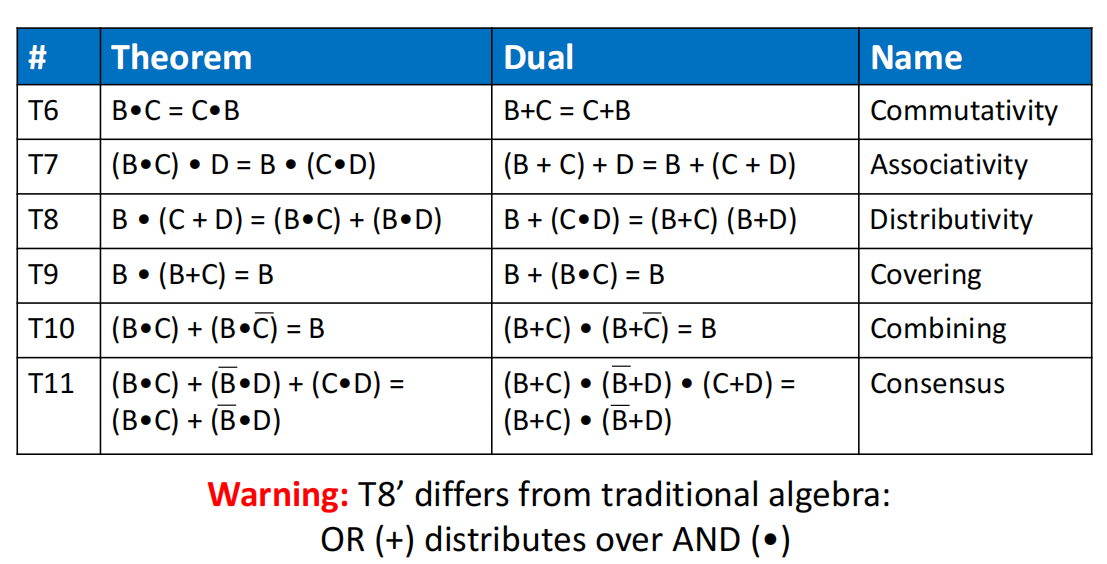
\includegraphics[width=\textwidth]{BooleanTheorems.png}
\subsubsection{Simplification methods}
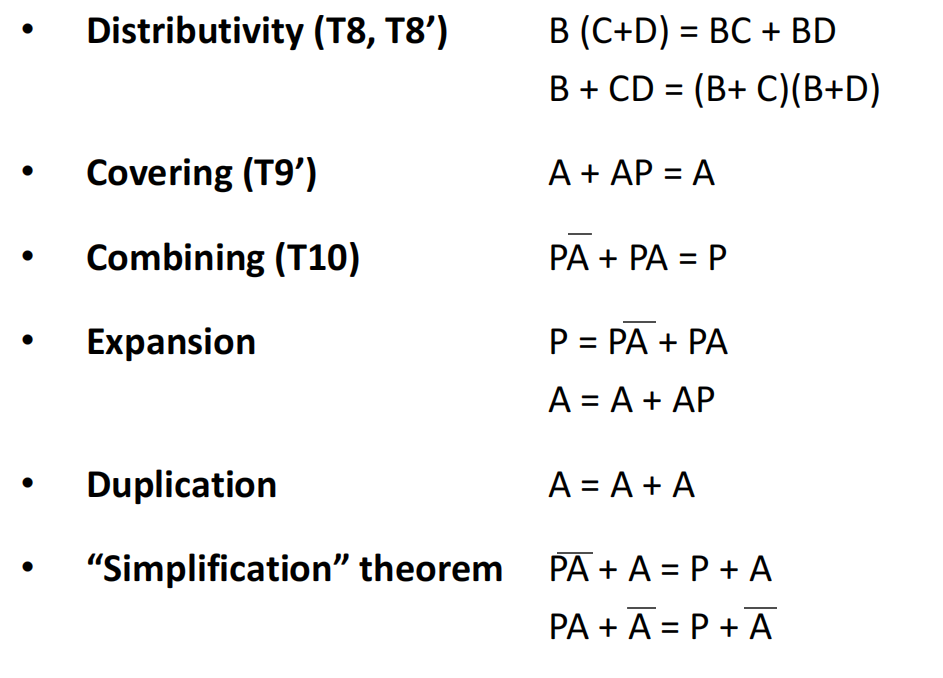
\includegraphics[width=\textwidth]{Simplification.png}
\subsection{K-Maps}
$PA+P \overline{A}=P$
\newline
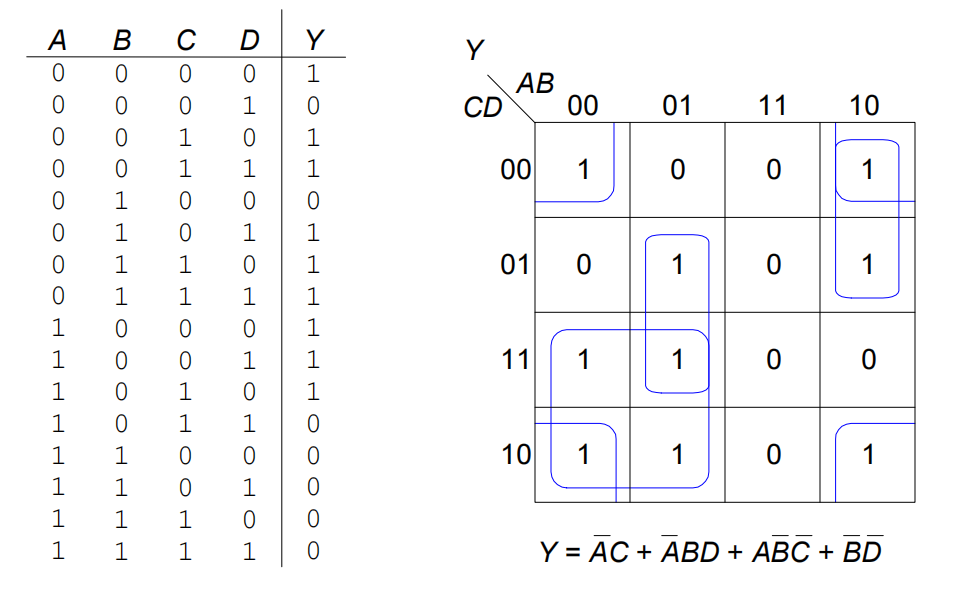
\includegraphics[width=\textwidth]{KMAPExample.png}
\subsection{Combinational Building Blocks}
\subsubsection{Mutiplexers}
$\lg_{2}^{N}$bit select input
\newline
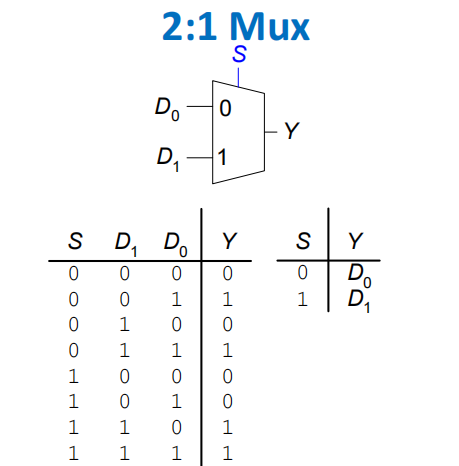
\includegraphics[width=\textwidth]{Mux.png}
\begin{itemize}
    \item Logic use
\end{itemize}
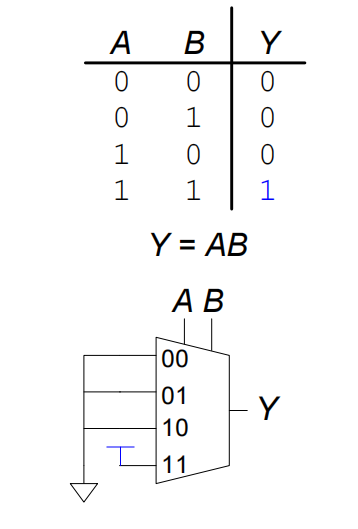
\includegraphics[width=0.5\textwidth]{LogicMux.png}
\subsubsection{Decoders}
$N$ inputs, $2^N$ outputs
\newline
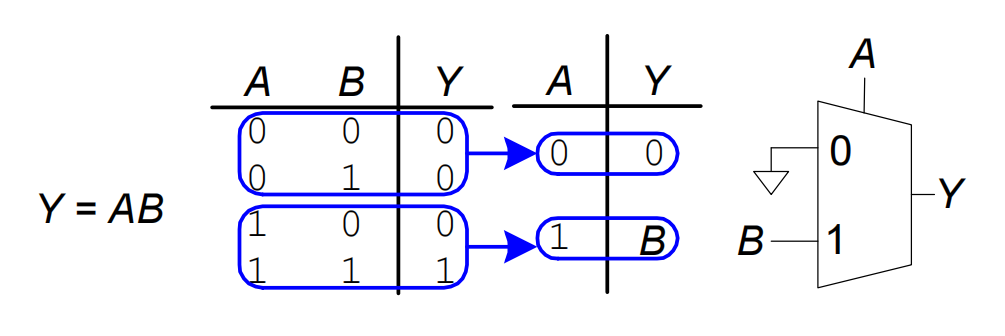
\includegraphics[width=\textwidth]{Decoder.png}
\begin{itemize}
    \item Logic use
\end{itemize}
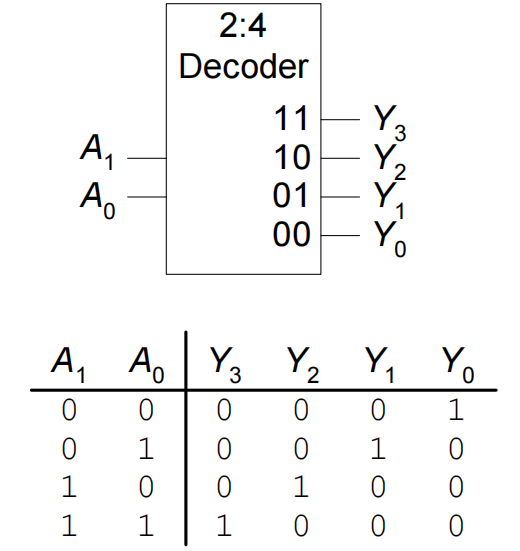
\includegraphics[width=0.5\textwidth]{LogicDecoder.png}
\subsection{Timing}
Because of wire resistance and we need time to fully charge the capacity
\begin{itemize}
    \item $t_{pd}$Propagation delay: the time from input starting to change to output becoming stable
    \item $t_{cd}$Contamination delay: the time from input starting to change to output starting to change
\end{itemize}
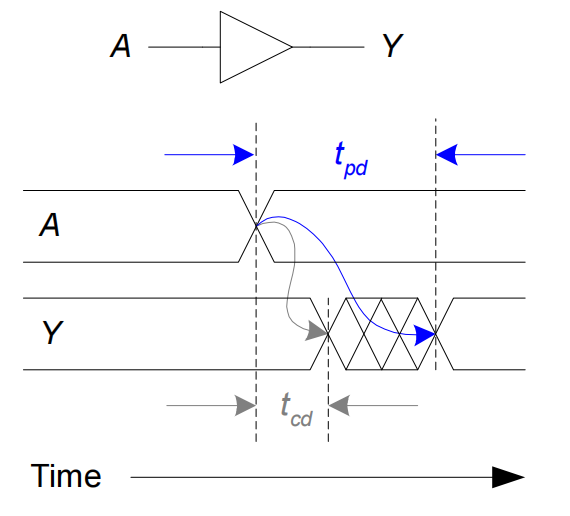
\includegraphics[width=0.8\textwidth]{Delay.png}
\begin{itemize}
    \item Different rising and falling delays
    \item multiple inputs and outputs
    \item circuits slow down when hot
\end{itemize}
\subsection{Critical paths}
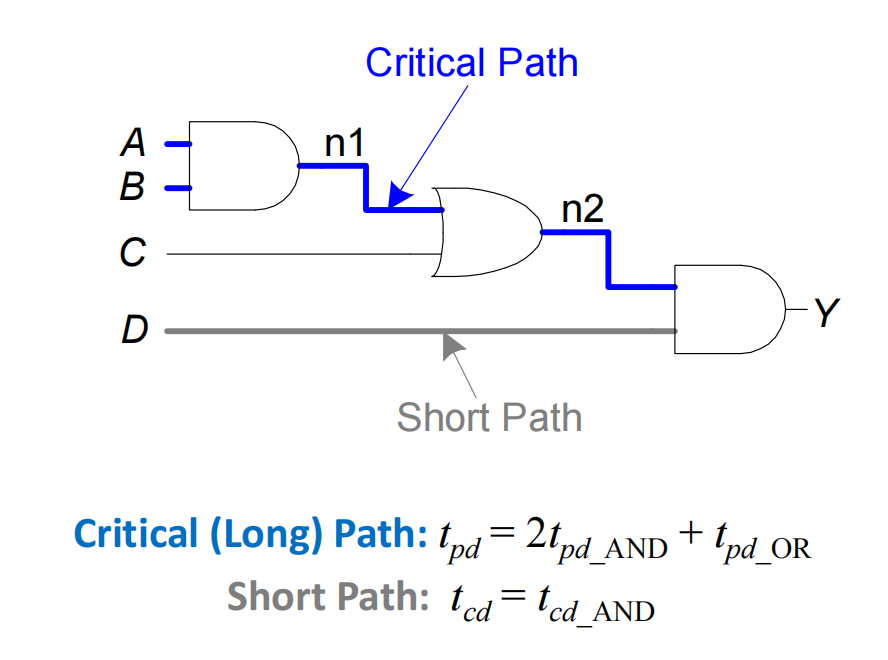
\includegraphics[width=0.8\textwidth]{CriticalPath.png}
\subsection{Glitches}
When a single input changes causes an output to change several times

\subsection{Sequential Logic}
\subsubsection{Definitions}
\begin{itemize}
    \item State: influence the future behavior
    \item Latches and flip-flops
    \item Synchronous sequential circuits
\end{itemize}
\subsection{State elements}
\subsubsection{Bistable Circuit}
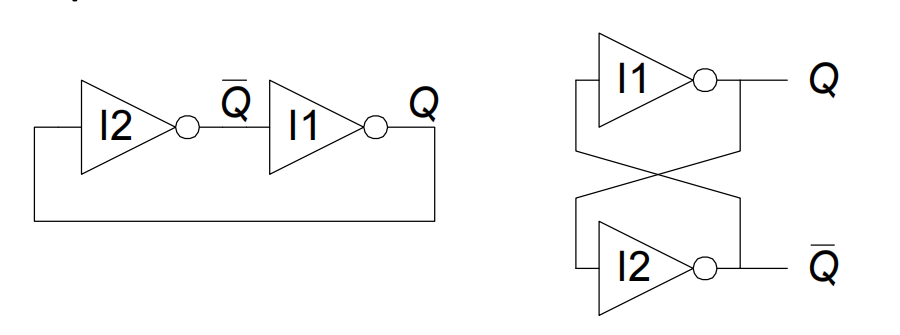
\includegraphics[width=0.8\textwidth]{Bistatble.png}
\subsubsection{SR Latch}
S: set, R: reset
\begin{itemize}
    \item S: 0, R: 0: previous
    \item S: 1, R: 0: 1
    \item S: 0, R: 1: 0
    \item S: 1, R: 1: invalid
\end{itemize}
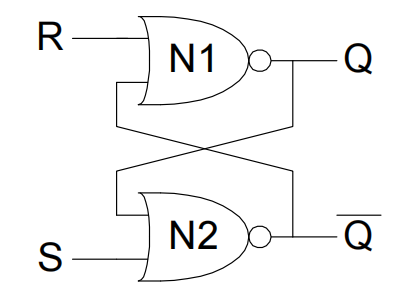
\includegraphics[width=0.5\textwidth]{SRLatch.png}
\subsubsection{D Latch}
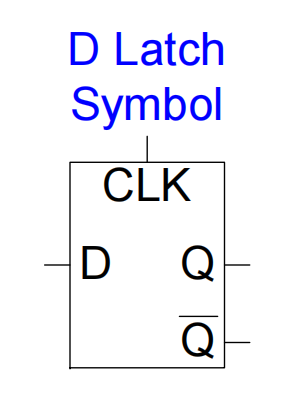
\includegraphics[width=0.5\textwidth]{DLatch.png}
\begin{itemize}
    \item CLK: controls when the output changes
    \item D: controls what the output changes to 
\end{itemize}
\subsubsection{D Flip-Flop}
Samples D on rising edge of CLK
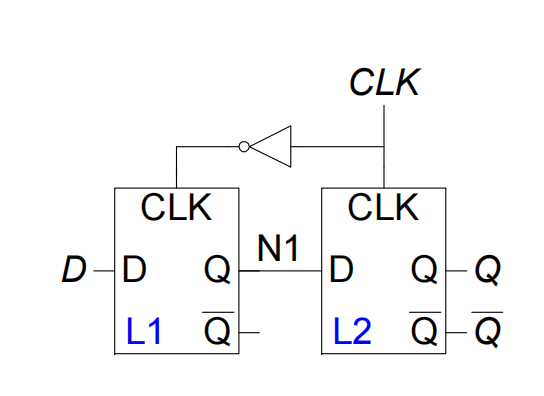
\includegraphics[width=0.5\textwidth]{DFlipFlop.png}

\subsection{Timing}
\subsubsection{Input timing constraint}
\begin{itemize}
    \item $t_{setup}$: time before clock edge data must be stable
    \item $t_{hold}$: time after clock edge data must be stable
    \item Aperture time$t_a$: time around clock edge data must be stable
\end{itemize}
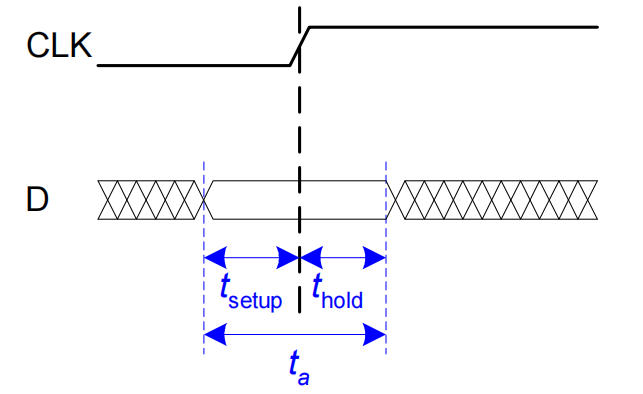
\includegraphics[width=0.5\textwidth]{InputTimeConstraint.png}
\subsubsection{Output timing constraint}
\begin{itemize}
    \item $t_{pcq}$: time after clock edge that the output Q is guaranteed to be stable
    \item $t_{ccq}$: time after clock edge data might be unstable
\end{itemize}
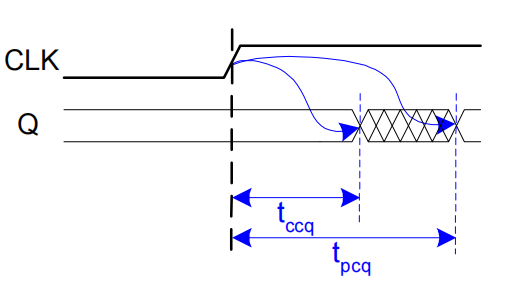
\includegraphics[width=0.5\textwidth]{OutputTimeConstraint.png}
\subsubsection{Setup Time Constraint}
\begin{itemize}
    \item input to register R2 must be stable at least $t_{setup}$ before clock edge
    \item clock edge time > Q be stable time + propagation time + set up time
    \item $T_c \geq t_{pcq} + t_{pd} + t_{setup}$
    \item $t_{pd} \leq T_c - (t_{pcq} + t_{setup})$
\end{itemize}
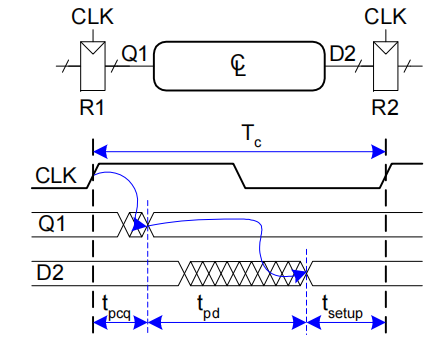
\includegraphics[width=0.5\textwidth]{ConstraintA.png}
\subsubsection{Hold Time Constraint}
\begin{itemize}
    \item input to register R2 must be stable at least $t_{hold}$ after clock edge
    \item hold time < Q1 starts to change time + D2 starts to change time
    \item $t_{hold} < t_{ccq} + t_{cd}$
    \item $t_{cd} > t_{hold} - t_{ccq}$
\end{itemize}
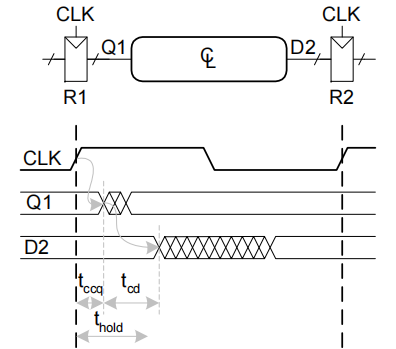
\includegraphics[width=0.5\textwidth]{ConstraintB.png}
\subsection{Clock Skew}
\begin{itemize}
    \item Skew: difference between two clock edges
    \item Perform worst case analysis to guarantee dynamic discipline is not violated for any register
\end{itemize}
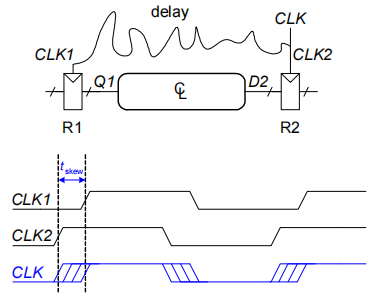
\includegraphics[width=0.5\textwidth]{ClockSkew.png}
\subsubsection{Setup Time Constraint with Skew}
\begin{itemize}
    \item in worst case, CLK2 is earilier than CLK1
    \item $T_c \geq t_{pcq} + t_{pd} + t_{setup} + t_{skew}$
    \item $t_{pd} \leq T_c - (t_{pcq} + t_{setup} + t_{skew})$
\end{itemize}
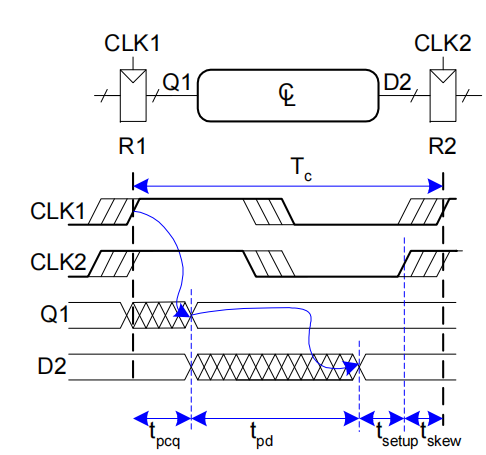
\includegraphics[width=0.5\textwidth]{ConstraintC.png}
\subsubsection{Hold Time Constraint with Skew}
\begin{itemize}
    \item in worst case, CLK2 is later than CLK1
    \item $t_{hold} + t_{skew} < t_{ccq} + t_{cd}$
    \item $t_{cd} > t_{hold} + t_{skew} - t_{ccq}$
\end{itemize}
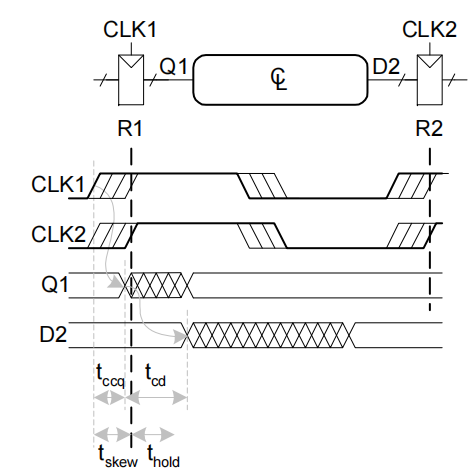
\includegraphics[width=0.5\textwidth]{ConstraintD.png}

\section{Pipeline Overview}
\subsection{Simple Processor Pipeline}
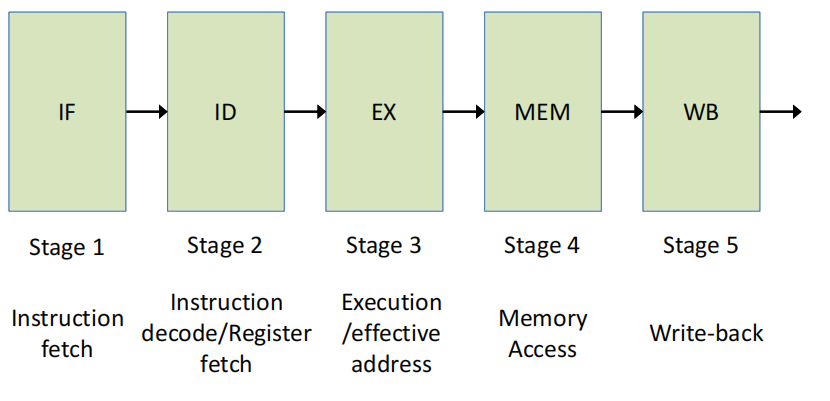
\includegraphics[width=0.8\textwidth]{SimpleProcessorPipeline.png}
\subsection{Five-Stage Pipeline for a RISC processor}
\begin{itemize}
    \item IF(Instruction Fetch)
    \item ID(Instruction Decode/Register Fetch)
    \item EX(Execution/Effective address)
    \item MEM(Memorry access): store instruction
    \item WB(Write-back): write the result back into the REGISTER FILE
\end{itemize}
\subsection{CPU Block Diagram}
\subsection{Hurdles in Pipelining}
\subsubsection{Structural Hazard: Resources}
\begin{itemize}
    \item All the overlapped instructions in pipeline requires pipelining of functional units and duplication of resources
    \item Resource conflict can happen when some combination of instructions cannot be accommodated.
\end{itemize}
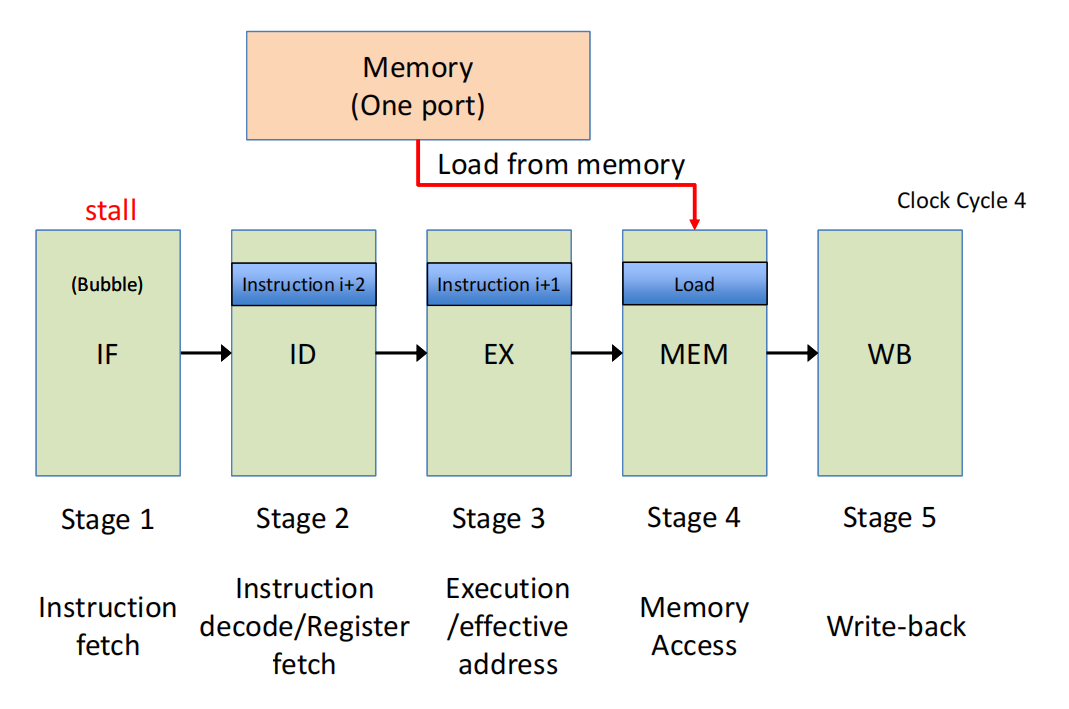
\includegraphics[width=0.8\textwidth]{StucturalHazard1.png}
\subsubsection{Data Hazard: Data dependency}
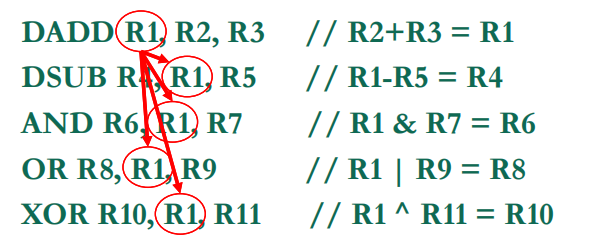
\includegraphics[width=0.5\textwidth]{DataHazard.png}
\begin{itemize}
    \item All the instructions after the DADD use the result of DADD
    \item The value of R1 is ready at WB stage of DADD, but DSUB needs it at its ID stage
\end{itemize}
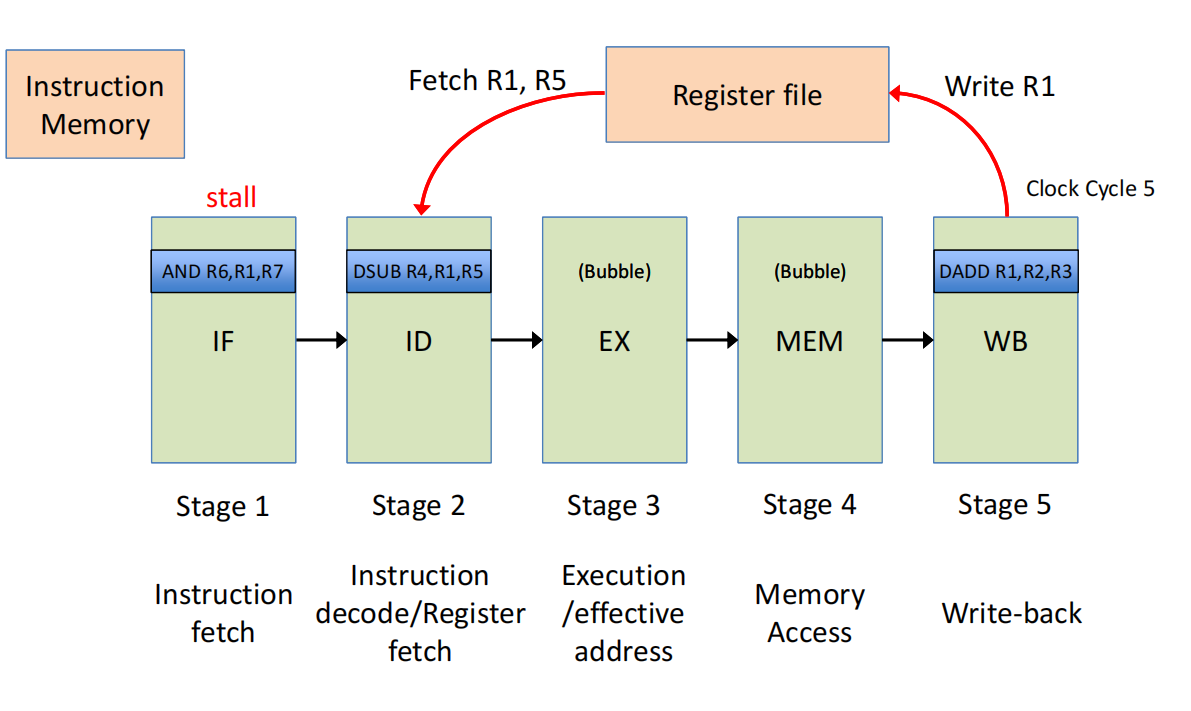
\includegraphics[width=0.8\textwidth]{StucturalHazard2.png}
\subsubsection{Control Hazard: Branch}
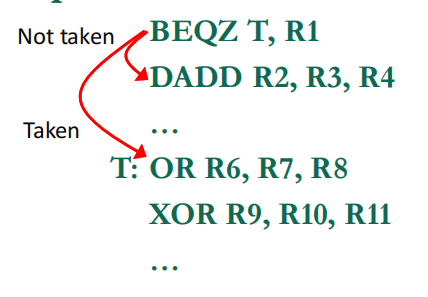
\includegraphics[width=0.5\textwidth]{ControlHazard.png}
\begin{itemize}
    \item Branch may change or not change the PC
    \item Which instruction to fetch after the branch?
    \item IF stalls until the branch condition is evaluated.
\end{itemize}
\subsection{Data Dependency}
\begin{itemize}
    \item True-dependence(pure-dependence, flow-dependence): an instruction depends on the result of a previous instruction
    \item Anti-dependence: an instruction requires a value that is later updated(because we are not executing instructions in order)
    \item Output-dependence: the ordering of instructions affects the final ouput result
\end{itemize}
\subsection{Out-of-order pipelnine}
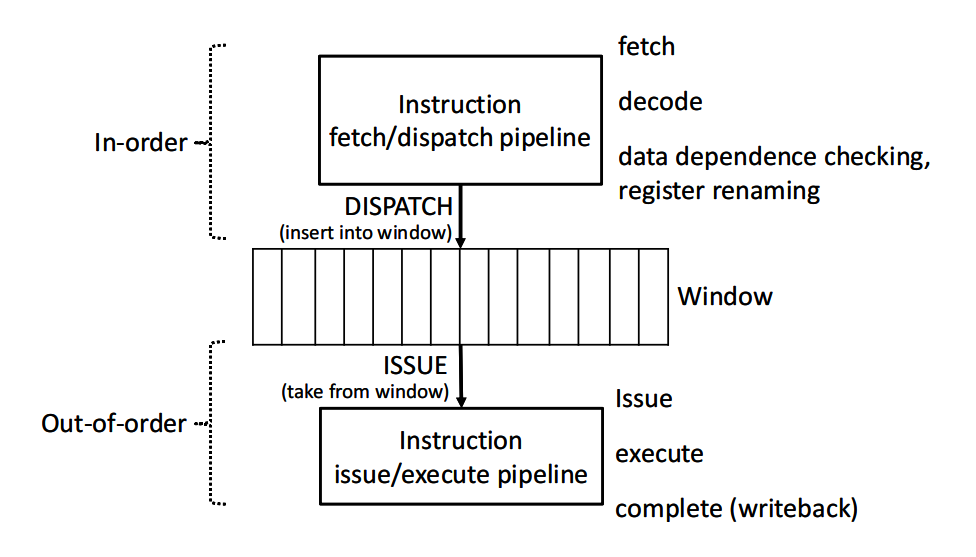
\includegraphics[width=\textwidth]{Out-of-orderPipelnine.png}
\begin{itemize}
    \item Instruction fetching do its job in order.
    \item Then put these instructions into a window
    \item When a instruction in the window gets ready, execute pipeline executes it
\end{itemize}
\subsection{Memory Wall}
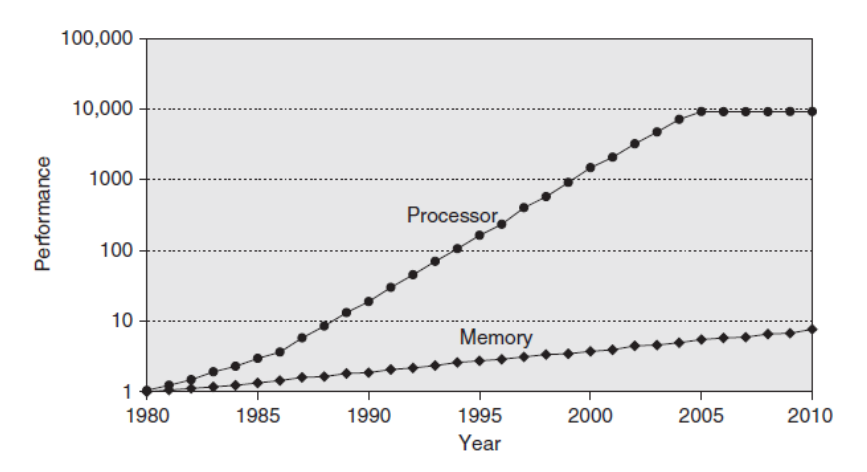
\includegraphics[width=0.8\textwidth]{MemoryWall.png}
\begin{itemize}
    \item Reason: The growing disparity of speed between CPU and main memory
    \item Given this trend, memory would become a performance bottleneck
\end{itemize}
\subsection{Memory Hierarchy Design}
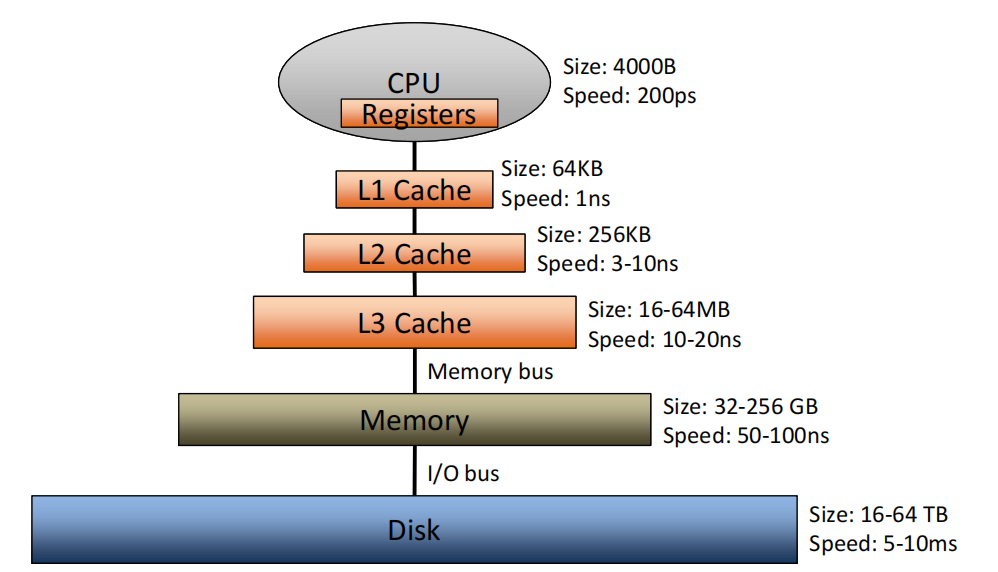
\includegraphics[width=0.8\textwidth]{MemoryHierarchy.png}
\begin{itemize}
    \item Large memory is slow
    \item processor wants large and fast memory
    \item Solution: take advantage of locality
\end{itemize}


\end{document}